% Beamer slide template prepared by Tom Clark <tom.clark@op.ac.nz>
% Otago Polytechnic
% Dec 2012

\documentclass[10pt]{beamer}
\usetheme{Dunedin}
\usepackage{graphicx}
\usepackage{fancyvrb}

\newcommand\codeHighlight[1]{\textcolor[rgb]{1,0,0}{\textbf{#1}}}

\title{Introduction to DNS}

\author[IN715]{Networks Administration}
\institute[Otago Polytechnic]{
  Otago Polytechnic \\
  Dunedin, New Zealand \\
}
\date{}
\begin{document}

%----------- titlepage ----------------------------------------------%
\begin{frame}[plain]
  \titlepage
\end{frame}


%----------- slide --------------------------------------------------%
\begin{frame}
  \frametitle{We all use DNS}

 \begin{itemize}
  \item If you want to communicate with a remote host over the Internet, 
        you need to know its IP address.
  \item For example the address for www.op.ac.nz is 202.49.5.68.
  \item We all know that we use the Domain Name System to find the 
        address for a given name.
  \item But how does this work, really? 
 \end{itemize}

\end{frame}


%----------- slide --------------------------------------------------%
\begin{frame}
  \frametitle{How did we get the name www.op.ac.nz?}

 \begin{itemize}
  \item Anything in the .nz zone is overseen by the Domain Name Commission (dnc.org.nz).
  \item The DNZ delegates the ability to register domain names to various authorised \emph{registrars}.
  \item An organisation like the the the Polytech registers its desired domain name with a registrar.
  \item It can then identify hostnames under the domain, like www.op.ac.nz, or it can further divide the zone into subdomains, like ict.op.ac.nz.
 \end{itemize}

\end{frame}

%----------- slide --------------------------------------------------%
\begin{frame}
  \frametitle{How do we get from www.op.ac.nz to 202.49.5.68?}

 That's a bit more complicated.  We have to create a record in DNS.  DNS is a
 \begin{itemize}
  \item Distributed,
  \item Hierarchical,
  \item Client-server,
  \item Directory system.
 \end{itemize}

\end{frame}

%----------- slide --------------------------------------------------%
\begin{frame}
  \frametitle{The DNS Hierarchy}

 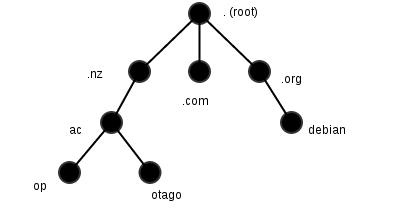
\includegraphics[scale=0.6]{dns.png}

\end{frame}



%----------- slide --------------------------------------------------%
\begin{frame}
  \frametitle{DNS Servers}

 \begin{itemize}
  \item To make all this work, we need DNS servers at each level of the 
        hierarchy.
  \item There are basically two ways in which a server may know the answer
        to a DNS query:
        \begin{enumerate}
          \item it may be \emph{authoritative} for the domain in question;
          \item it may perform a \emph{recursive} lookup.
        \end{enumerate}
  \item If a DNS server is not authoritative and it doesn't perform recursive
        lookups, it will provide a referral to another DNS server that may
        know the answer.
 \end{itemize}

\end{frame}

%----------- slide --------------------------------------------------%
\begin{frame}
  \frametitle{DNS Clients}

 
 \begin{itemize}
  \item A client machine that needs to perform a DNS lookup uses its
        \emph{resolver}
  \item A resolver may be a local service, but typically it is a system 
        library.
 \end{itemize}

\end{frame}



%----------- slide --------------------------------------------------%
\begin{frame}
  \frametitle{The lookup process}

 Suppose a DNS client makes a recursive query for the address of
 kate.ict.op.ac.nz, and the server receiving the query is not authoritative
 and does not have any relevant cached information.
 \begin{enumerate}
  \item It starts by querying a \emph{root} server to find the address of
        a DNS server that is authoritative for .nz.
  \item It queries that server to find one that is authoritative for ac.nz.
  \item It queries that server to find one that is athoritative for op.ac.nz.
  \item It is finally referred to a server that is authoritative for ict.op.ac.z, and that server responds with an address for kate.
 \end{enumerate}

\end{frame}



%----------- slide --------------------------------------------------%
\begin{frame}[fragile]
  \frametitle{What about reverse lookups?}

 Suppose we want to find the hostname for 202.49.5.60?

 \begin{verbatim}
     kate.ict.op.ac.nz.   The hierarchy goes right-to-left.
    
     202.49.5.60          The hierarchy goes left-to-right.
 \end{verbatim}

IP addresses don't match the hierarchical structure of DNS.
\end{frame}


%----------- slide --------------------------------------------------%
\begin{frame}
  \frametitle{The solution is to invert the hierarchy of IP addresses.}
   
  To find the hostname for 202.49.5.60, we look up 
  60.5.49.202.in-addr.addr.arpa.

\end{frame}


%----------- slide --------------------------------------------------%
\begin{frame}
  \frametitle{DNS Software}

 \begin{itemize}
  \item BIND: The de facto standard DNS server.
  \item dig, host: client tools useful for inspecting and troubleshooting
        DNS issues.
 \end{itemize}

\end{frame}

\end{document}
